\pagenumbering{arabic}
\section{Introducción}

El cáncer es un término génerico para describir una variedad de enfermedades que pueden afectar a cualquier parte del organismo. Este está definido por el crecimiento descontrolado de células anormales. Estas pueden invadir otros organismos por medio de un proceso que se llama <<metástasis>> \cite{cancer_gov_que_es}. La Organización Mundial de la Salud afirma que el cáncer es una de las principales causas de muerte en todo el mundo, causando al rededor de 10 millones de defunciones en todo el mundo \cite{who_cancer_2022}. Tan solo en México, en 2023 hubo 799,869 defunciones de las cuales el 11.4\% fueron por tumores malignos según datos de la INEGI \cite{INEGI2025}

El tumor cerebral maligno es una de las enfermedades más peligrosas debido a su mal pronóstico y a las dificultades inherentes a su tratamiento. Un obstáculo clave es la barrera hematoencefálica (BHE), que limita la eficacia de los paradigmas diagnósticos y terapéuticos. En respuesta, la comunidad científica busca activamente soluciones innovadoras; trabajos como los de Ijaz et al. y Hasan et al. son ejemplos de esfuerzos dedicados a desarrollar sondas de diagnóstico avanzadas y nanomedicinas para mejorar la detección temprana y el tratamiento de estos tumores \cite{ijaz_diagnostics_2025, hasan_recent_2023}. Aun que los tumores trabajados en este proyecto son benignos, la detección temprana de estos es crucial para prevenir su progresión a malignidad y mejorar el pronóstico del paciente. También el trabajo hecho se podría replicar para verificar su eficacia en tumores malignos.


En este contexto, el diagnóstico temprano y preciso mediante IRM se ha consolidado como un pilar fundamental en la neurooncología moderna, ya que influye directamente en la eficacia del tratamiento y el pronóstico del paciente \cite{Akkus2017deep}. En los últimos años, la inteligencia artificial, y en particular los modelos de aprendizaje profundo, han revolucionado la interpretación de estas imágenes, alcanzando niveles de precisión en la detección de tumores comparables a los de radiólogos expertos \cite{pereira2016brain, liew2018artificial}. Modelos avanzados como BrainTumorSegNet \cite{XiaojunHu2020} y qER de Qure.ai \cite{Qure.ai2024} ejemplifican este éxito. Sin embargo, la aplicabilidad de estos enfoques clásicos enfrenta dos barreras significativas: la dependencia de enormes volúmenes de datos para el entrenamiento y la necesidad de una alta capacidad de cómputo. Estas limitaciones restringen su implementación en entornos clínicos con recursos computacionales limitados y pueden ralentizar la optimización de los modelos. Ante este panorama, emerge la siguiente pregunta de investigación: ¿Es posible desarrollar un modelo de clasificación de imágenes de IRM que mantenga una alta precisión diagnóstica reduciendo al mismo tiempo la dependencia de recursos computacionales masivos?

\subsection*{Sumario de la Revisión de la Literatura y Justificación del Estudio}

\justify
Para abordar las limitaciones mencionadas, esta investigación explora la computación cuántica como una alternativa disruptiva. A diferencia de los bits clásicos, los cúbits aprovechan los principios de superposición y entrelazamiento para procesar información de manera exponencialmente más potente, permitiendo que los algoritmos cuánticos resuelvan problemas de alta complejidad con menos recursos \cite{mcmahon2008}. En el campo del diagnóstico médico, ya existen propuestas que integran enfoques cuánticos y clásicos. Por ejemplo, el modelo HQC-CNN utiliza un circuito cuántico para la extracción de características en la clasificación de tumores cerebrales \cite{HQC-CNN}, mientras que otros han aplicado el aprendizaje por transferencia cuántico al diagnóstico de Alzheimer y Parkinson \cite{math11020376}. Un trabajo de referencia es el de Khan et al. \cite{khan2024brain}, quienes desarrollaron una red híbrida (HQCNN) que emplea codificación angular para clasificar tumores con una precisión del 91.4\%. Este estudio se justifica en la necesidad de superar los cuellos de botella computacionales de la IA clásica, proponiendo una arquitectura híbrida novedosa que no solo busca mejorar la precisión, sino también optimizar la eficiencia del procesamiento de datos médicos.

\subsection*{Objetivos e Hipótesis}

El objetivo general de esta investigación es desarrollar y evaluar una arquitectura de red neuronal híbrida cuántico-clásica para la clasificación de tumores cerebrales en imágenes de resonancia magnética, que demuestre un rendimiento superior en precisión y eficiencia computacional en comparación con enfoques híbridos existentes.

De este objetivo se desprende la siguiente hipótesis:
\textit{$H_1$: Una arquitectura de red híbrida que utiliza el algoritmo cuántico de extracción de características \textbf{Amplitude Encoding} (Codificación por Amplitud) \cite{nakaji2022approximate} junto con una red neuronal clásica, logrará una mayor precisión en la clasificación de imágenes de IRM que el modelo híbrido de Khan et al. \cite{khan2024brain}, el cual se basa en la codificación angular.}

\subsection*{Contexto, Variables y Términos Clave}

\justify
Esta investigación se realizará en un entorno de simulación computacional. Se utilizará un conjunto de datos público de imágenes de resonancia magnética cerebral \cite{cheng2017brain} para entrenar y validar los modelos. Este conjunto de datos es el mismo que utilizo Khan et al. \cite{khan2024brain} y servirá como base para comprobar nuestra hipótesis. El desarrollo de la arquitectura clásica se llevará a cabo con la librería PyTorch, mientras que los componentes cuánticos serán diseñados y simulados utilizando el kit de desarrollo de software Qiskit de IBM para Python. También se planea utilizar la plataforma en la nube IBM Quantum Experience para ejecutar simulaciones en hardware cuántico real, sin embargo estaremos sujetos a la disponibilidad y las limitaciones de acceso.

Las variables principales son:
\begin{itemize}
    \item \textbf{Variable Independiente}: La arquitectura del modelo de clasificación, comparando (a) el enfoque híbrido propuesto con \textit{Amplitude Encoding} y (b) el enfoque híbrido de referencia con codificación angular.
    \item \textbf{Variable Dependiente}: La precisión (\textit{accuracy}) del modelo en la tarea de clasificación binaria (presencia o ausencia de tumor).
\end{itemize}

\subsection*{Limitaciones de la Investigación y Utilidad del Estudio}

\justify
El estudio presenta dos limitaciones principales. Primero, el uso de simuladores cuánticos no refleja completamente las condiciones de ruido y decoherencia inherentes al hardware cuántico real, lo que podría afectar la generalización de los resultados. Segundo, la investigación se enfoca exclusivamente en una clasificación binaria, sin abordar tareas más complejas como la segmentación tumoral o la clasificación multiclase (e.g., glioma, meningioma). Segundo, el simulador de IBM Quantum Experience tiene limitaciones en cuanto al número de cúbits, la profundidad del circuito e incluso el tiempo que podemos utilizar, lo cual podría afectar seriamente nuestros resultados para cuando queramos comparar a hardware cuántico real.

A pesar de estas limitaciones, la utilidad de este estudio es doble. Para el campo académico, aporta evidencia sobre la viabilidad y el potencial de las técnicas de \textit{quantum machine learning}, específicamente del \textit{Amplitude Encoding}, en el dominio de imágenes médicas. A nivel profesional y clínico, los hallazgos podrían sentar las bases para el desarrollo de futuras herramientas de diagnóstico asistido por computadora que sean más rápidas, accesibles y eficientes, democratizando el acceso a tecnologías de diagnóstico avanzado en centros con infraestructura computacional modesta.


%%%%%%%%%%%%%%%%%%%%%%%%%%%%%%%%%%%%%%%%%
%%%%%%%%%%%%%ANTECEDENTES%%%%%%%%%%%%%%%%
%%%%%%%%%%%%%%%%%%%%%%%%%%%%%%%%%%%%%%%%%

\section{Antecedentes} 
    En la figura~\ref{fig:cicata edificio}  \lipsum[1]
    \begin{figure}
       \centering
        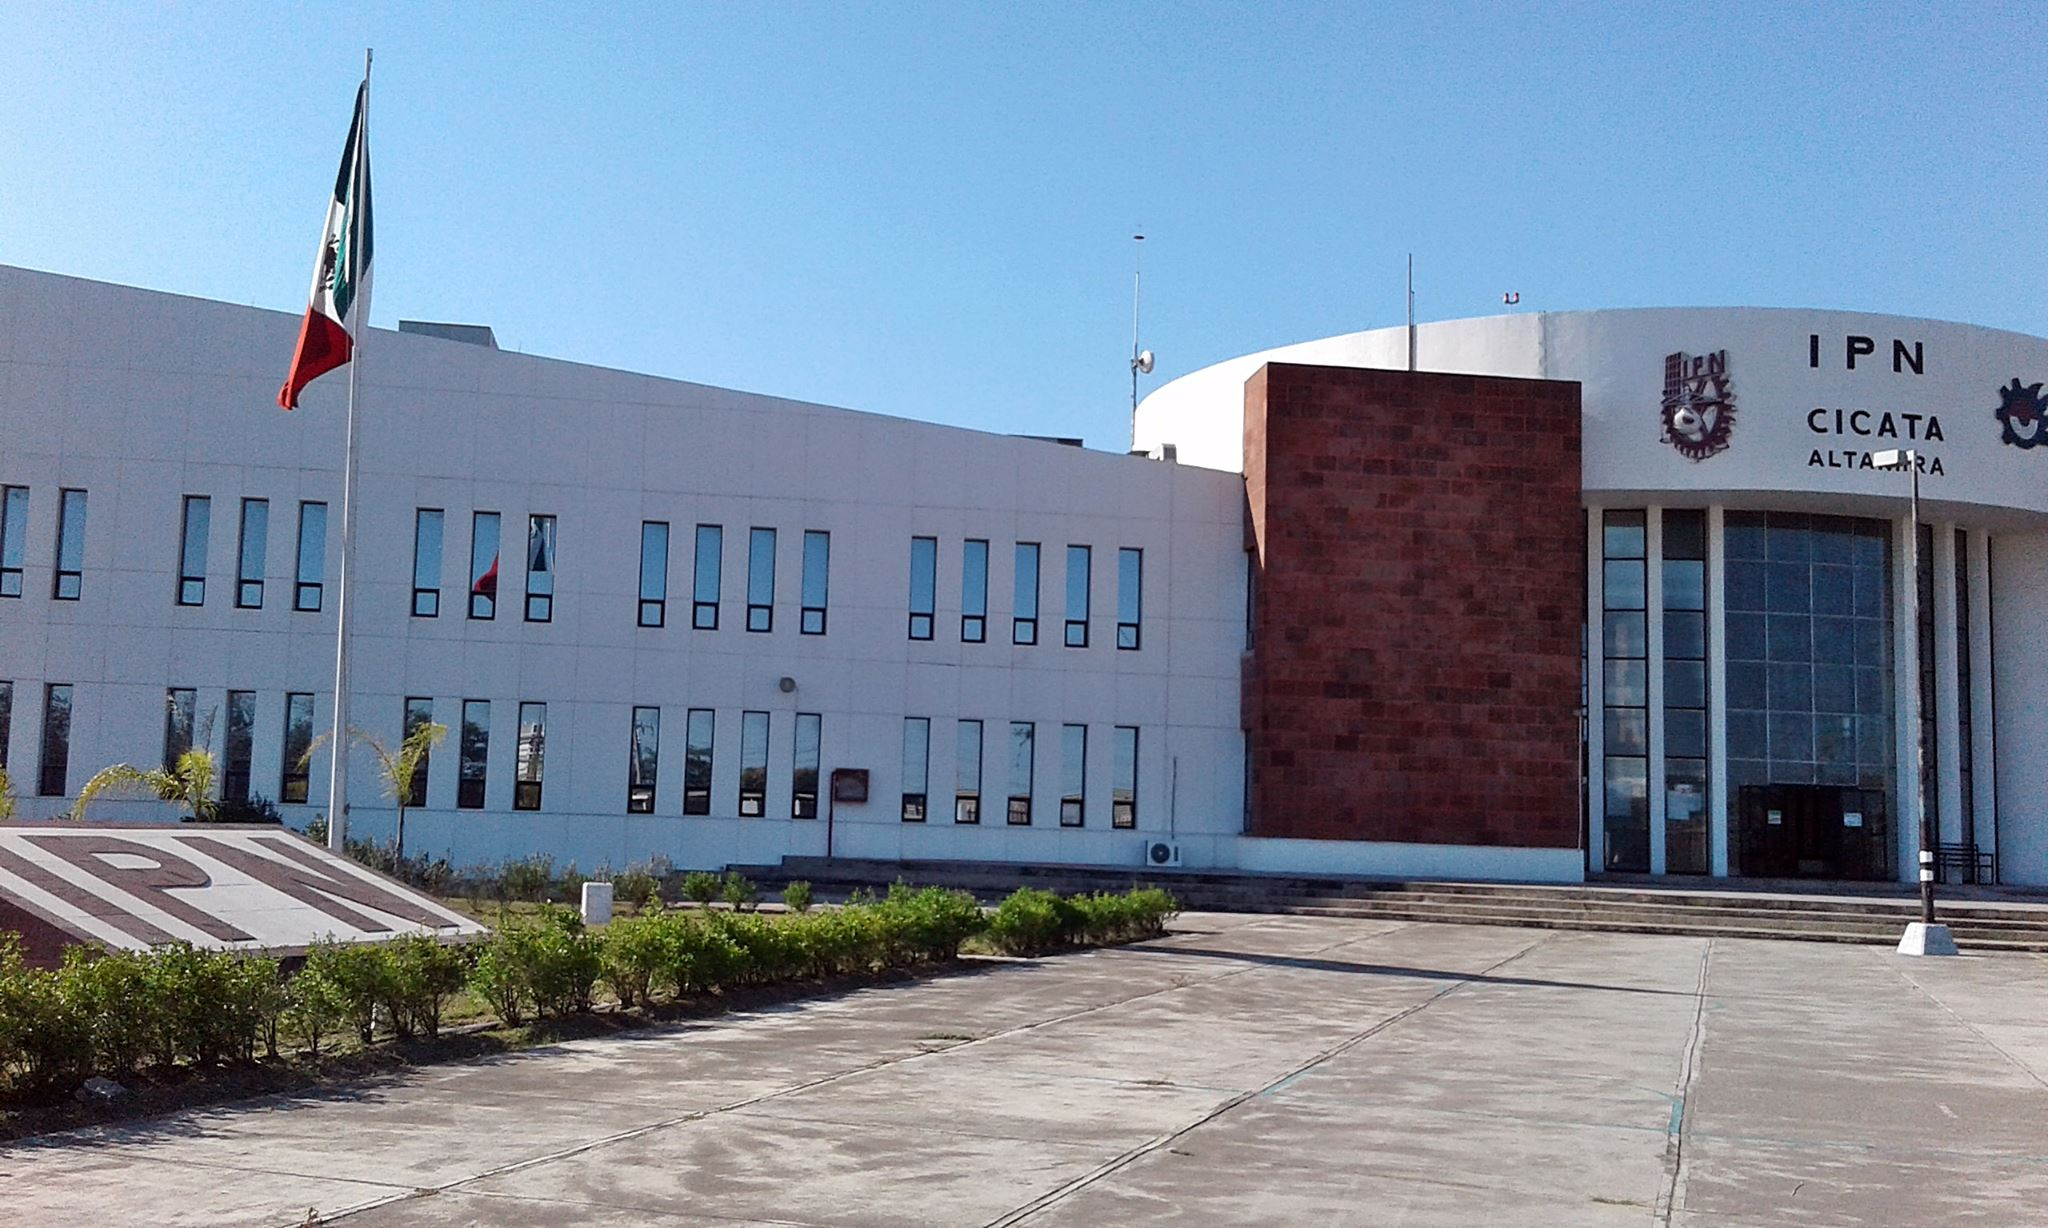
\includegraphics[width=1\textwidth]{src/images/cicata-alt-building.jpeg}
        \caption{Edificio principal de CICATA Altamira}
        \label{fig:cicata edificio}
    \end{figure}    

\section{Estado del arte}
    \lipsum[1]~\ref{tab:cicata-loc}

    \lipsum[2]
    \begin{table}[h]
    \centering
    \caption{Centros de Investigación en Ciencia Aplicada y Tecnología Avanzada del IPN en México}
    \vspace{0.3cm}
    \begin{tabular}{ccc}
        \hline
        \textbf{Nombre} & \textbf{Ubicación} & \textbf{Áreas de Especialización} \\ \hline
        CICATA Altamira & Altamira, Tamaulipas & Materiales Avanzados \\
        CICATA Legaria & Ciudad de México & Innovación Tecnológica \\
        CICATA Querétaro & Querétaro, Querétaro & Nanotecnología \\ 
        CICATA Reynosa & Reynosa, Tamaulipas & Ingeniería de Software \\ 
        CICATA Unidad IPN Ticomán & Ciudad de México & Electrónica, Física Aplicada \\ \hline
    \end{tabular}
    \label{tab:cicata-loc}
\end{table}


    \cite{garcia2024exploration}~\lipsum[3]


\section{Justificación}
    \lipsum[1]

\section{Objetivo general}
    Phasellus eu tellus sit amet tortor gravida placerat. Integer sapien est, iaculis in, pretium quis, viverra ac, nunc. Praesent eget sem vel leo ultrices bibendum. Aenean faucibus. Morbi dolor nulla, malesuada eu, pulvinar at, mollis ac, nulla. 

\section{Objetivos especificos}
    \begin{enumerate}
        \item Curabitur dictum gravida mauris. Nam arcu libero, nonummy eget, consectetuer id, vulputate a, magna. 
        \item Raesent eget sem vel leo ultrices bibendum. Aenean faucibus. Morbi dolor nulla, malesuada eu, pulvinar at, mollis ac, nulla
        \item CDuis nibh mi, congue eu, accumsan eleifend, sagittis quis, diam. Duis eget orci sit amet orci dignissim rutrum.
    \end{enumerate}